\section{Date: 2026-10-18}
\noindent \textbf{Series ID: DEXSIUS} 

\noindent This series is titled Singapore Dollars to U.S. Dollar Spot Exchange Rate and has a frequency of Daily. The units are Singapore Dollars to One U.S. Dollar and the seasonal adjustment is Not Seasonally Adjusted.The observation start date is 1981-01-02 and the observation end date is 2026-10-09.The popularity of this series is 43. \\ 

\noindent \textbf{Series ID: ATNHPIUS12060Q} 

\noindent This series is titled All-Transactions House Price Index for Atlanta-Sandy Springs-Alpharetta, GA (MSA) and has a frequency of Quarterly. The units are Index 1995:Q1=100 and the seasonal adjustment is Not Seasonally Adjusted.The observation start date is 1975-10-01 and the observation end date is 2024-10-01.The popularity of this series is 31. \\ 

\subsection{Raw Regression}
\noindent Regresses the two series against each other directly. A significant result here can come just as easily from both series sharing a long-run trend as from any real relationship.

\begin{center}
\begin{tabular}{lclc}
\toprule
\textbf{Dep. Variable:}       & value\_fred\_ATNHPIUS12060Q & \textbf{  R-squared:         } &     0.397   \\
\textbf{Model:}               &             OLS             & \textbf{  Adj. R-squared:    } &     0.390   \\
\textbf{Method:}              &        Least Squares        & \textbf{  F-statistic:       } &     61.19   \\
\textbf{Date:}                &       Sun, 18 Oct 2026      & \textbf{  Prob (F-statistic):} &  7.95e-12   \\
\textbf{Time:}                &           14:58:04          & \textbf{  Log-Likelihood:    } &   -516.90   \\
\textbf{No. Observations:}    &                95           & \textbf{  AIC:               } &     1038.   \\
\textbf{Df Residuals:}        &                93           & \textbf{  BIC:               } &     1043.   \\
\textbf{Df Model:}            &                 1           & \textbf{                     } &             \\
\textbf{Covariance Type:}     &          nonrobust          & \textbf{                     } &             \\
\bottomrule
\end{tabular}
\begin{tabular}{lcccccc}
                              & \textbf{coef} & \textbf{std err} & \textbf{t} & \textbf{P$> |$t$|$} & \textbf{[0.025} & \textbf{0.975]}  \\
\midrule
\textbf{const}                &     388.3669  &       31.303     &    12.407  &         0.000        &      326.205    &      450.529     \\
\textbf{value\_fred\_DEXSIUS} &    -147.6593  &       18.876     &    -7.822  &         0.000        &     -185.144    &     -110.175     \\
\bottomrule
\end{tabular}
\begin{tabular}{lclc}
\textbf{Omnibus:}       & 33.207 & \textbf{  Durbin-Watson:     } &    0.045  \\
\textbf{Prob(Omnibus):} &  0.000 & \textbf{  Jarque-Bera (JB):  } &   59.548  \\
\textbf{Skew:}          &  1.439 & \textbf{  Prob(JB):          } & 1.17e-13  \\
\textbf{Kurtosis:}      &  5.599 & \textbf{  Cond. No.          } &     12.1  \\
\bottomrule
\end{tabular}
%\caption{OLS Regression Results}
\end{center}

Notes: \newline
 [1] Standard Errors assume that the covariance matrix of the errors is correctly specified.

\begin{figure}
\centering
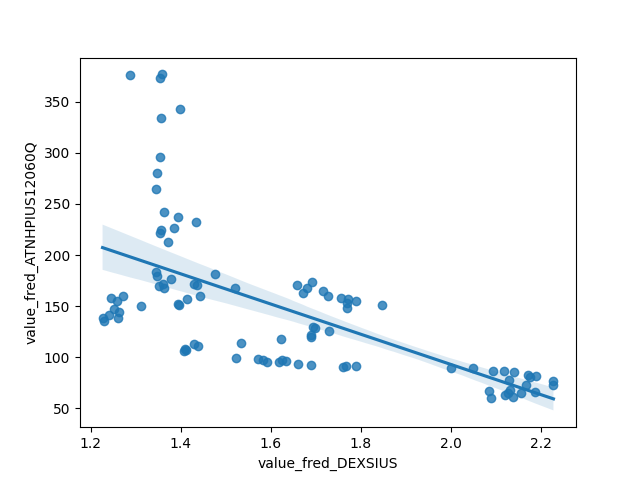
\includegraphics[scale = 0.9]{plots/plot_2026-10-18.png}
\caption{Raw Regression Plot for 2026-10-18}
\end{figure}
\newpage
\subsection{Detrended Regression}
\noindent Regresses the residuals of each series after removing its own linear time trend, so a shared trend can no longer drive the result on its own. A relationship that stays significant here is better evidence of a genuine link between the two series.

\begin{center}
\begin{tabular}{lclc}
\toprule
\textbf{Dep. Variable:}                  & value\_fred\_ATNHPIUS12060Q\_detrended & \textbf{  R-squared:         } &     0.271   \\
\textbf{Model:}                          &                  OLS                   & \textbf{  Adj. R-squared:    } &     0.264   \\
\textbf{Method:}                         &             Least Squares              & \textbf{  F-statistic:       } &     34.66   \\
\textbf{Date:}                           &            Sun, 18 Oct 2026            & \textbf{  Prob (F-statistic):} &  6.19e-08   \\
\textbf{Time:}                           &                14:58:04                & \textbf{  Log-Likelihood:    } &   -455.29   \\
\textbf{No. Observations:}               &                     95                 & \textbf{  AIC:               } &     914.6   \\
\textbf{Df Residuals:}                   &                     93                 & \textbf{  BIC:               } &     919.7   \\
\textbf{Df Model:}                       &                      1                 & \textbf{                     } &             \\
\textbf{Covariance Type:}                &               nonrobust                & \textbf{                     } &             \\
\bottomrule
\end{tabular}
\begin{tabular}{lcccccc}
                                         & \textbf{coef} & \textbf{std err} & \textbf{t} & \textbf{P$> |$t$|$} & \textbf{[0.025} & \textbf{0.975]}  \\
\midrule
\textbf{const}                           &   -7.456e-12  &        3.026     & -2.46e-12  &         1.000        &       -6.010    &        6.010     \\
\textbf{value\_fred\_DEXSIUS\_detrended} &     113.8433  &       19.338     &     5.887  &         0.000        &       75.441    &      152.245     \\
\bottomrule
\end{tabular}
\begin{tabular}{lclc}
\textbf{Omnibus:}       & 35.396 & \textbf{  Durbin-Watson:     } &    0.076  \\
\textbf{Prob(Omnibus):} &  0.000 & \textbf{  Jarque-Bera (JB):  } &   73.595  \\
\textbf{Skew:}          &  1.434 & \textbf{  Prob(JB):          } & 1.04e-16  \\
\textbf{Kurtosis:}      &  6.220 & \textbf{  Cond. No.          } &     6.39  \\
\bottomrule
\end{tabular}
%\caption{OLS Regression Results}
\end{center}

Notes: \newline
 [1] Standard Errors assume that the covariance matrix of the errors is correctly specified.

\begin{figure}
\centering
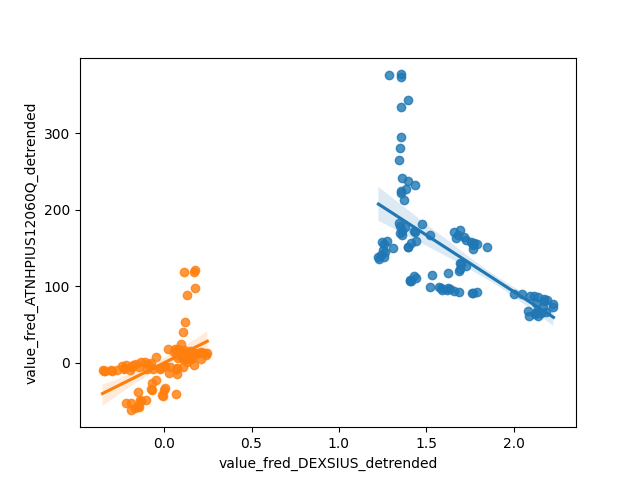
\includegraphics[scale = 0.9]{plots/plot_2026-10-18_detrended.png}
\caption{Detrended Regression Plot for 2026-10-18}
\end{figure}
\newpage
